\chapter{Introdução} \label{sec:intro}

O objetivo deste trabalho consiste na compreensão de vários conceitos ligados ao \textbf{Routing}.

Primeiramente será feita uma avaliação teórica dos conceitos de \textbf{Routing Interior}, nomeadamente o protocolo \textbf{OSPF}.
Deste modo será criada com recurso aos sistemas de cada bancada de trabalho um \textbf{Autonomous System}.

A segunda parte do trabalho prende-se com a implementação de um protocolo de \textbf{Routing Exterior}, o \textbf{BGP}.
Este protocolo permitira a ligação aos diferentes AS das restantes bancadas, pelo que involve a cooperação dos restates colegas na sala.

\chapter{Fundamentos Teóricos} \label{sec:objectives}

\section{OSPF}

OSPF (\textit{Open Shortest Path First}) é um protocolo de \textit{routing} de internet TCP/IP \cite{ospf}.
Classifica-se como sendo um protocolo de \textit{routing} interior, partilhando deste modo informação entre todos os routers que pertencem ao mesmo AS (\textit{Autonomous System}).

Um \textbf{Autonomous System} é um conjunto de routers que comunicam entre e trocam informação através de um protocolo de \textit{routing} comum.
Deste modo, um AS está unificado na sua política de \textit{routing} ao exterior.

Este protocolo baseia-se no tecnologia \textit{link-state}.
Este abordagem implica que cada router tem guardada numa base de dados interna a tipologia de rede do AS.
Se estiver a operar corretamente, todos os routers têm que ter a mesma informação na base de dados.
A comunicação do estado das ligações aos restantes routers é feito através de \textit{flooding}, pelo que rapidamente é possível atualizar todas a bases de dados.

Devido a esta abordagem de comunicação dentro do AS, o OSPF classifica-se também como um \textbf{Protocolo de Routing Dinâmico}.
Quando a tipologia do AS é mudada, como por exemplo um router desligar-se, o sistema rapidamente deteta a falha.
Após um curto tempo de estabilização, associado à frequência com que as mensagens de sincronização HELLO são enviadas,
novas rotas são geradas e medidas de forma a apresentar a nova rota ótima, i.e., com o menor curto.

\begin{figure}[H]
    \centering
    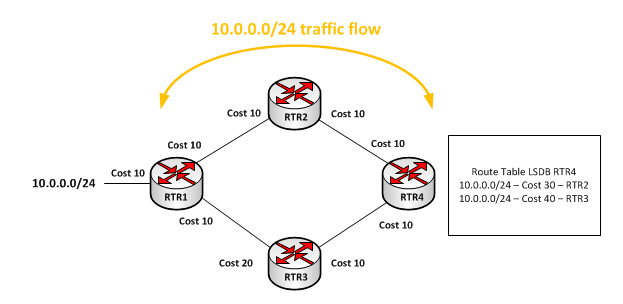
\includegraphics[width=.85\linewidth]{figs/intro/ospf_cost.png}
    \caption{Exemplo de tipologia de rede de um AS com custos associados}
    \label{fig:ospf_cost}
\end{figure}

O custo das rotas está associada à \textit{bandwidth} de cada ligação. Quando maior a largura de banda, menor será o custo da rota.
No caso de mais que uma rota ter o mesmo custo, no caso da CISCO, até um máximo de 6 opções são guardadas para o próximo \textit{hop}.

No exemplo apresentado, as duas rotas possíveis de RTR1 para RTR4 são:
\begin{itemize}
    \item Por RTR2, com custo de 20, rota ótima
    \item Por RTR3, com custo de 30, rota secundária
\end{itemize}

No caso do RTR2 deixar de funcionar, o sistema rapidamente iria atualizar e definir a rota pelo RTR3 com a melhor (e única) solução.


\section{BGP}

BGP (\textit{Border Gateway Protocol}) é um protocolo de \textit{routing} externo \cite{bgp}. 
Se com o OSPF definimos uma AS e as comunicações entre as diferentes \textit{networks} que dela fazem parte,
com BGP permite-se a comunicação entre AS de forma a partilhar informações sobre as \textit{networks} internas de cada AS.

Também é partilhada a informação sobre os AS que estão no caminho para comunicar com essas \textit{networks}.

Deste modo, é possível mapear toda a rede AS, e definir quais os caminhos ótimos para atingir cada AS.

\begin{figure}[H]
    \centering
    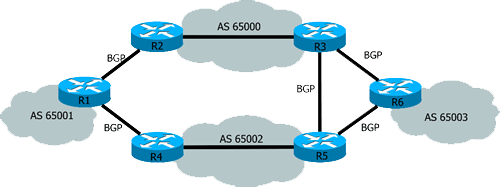
\includegraphics[width=.8\linewidth]{figs/intro/bgp_link.png}
    \caption{Exemplo de tipologia de rede com diferentes AS}
    \label{fig:bgp_link}
\end{figure}

Na tipologia exemplo acima apresentada, 4 AS estão interligados através de routers que suportam o protocolo BGP.
É de notar que por exemplo, o R5 tem 3 caminho diferentes possíveis para comunicar com o R3.
De forma similar ao \textbf{OSPF}, no caso de falha de uma ligação, o sistema é capaz de se adaptar e criar novas rotas.